\setcounter{page}{2}
\section*{Цель работы}
На базе предложенного шаблона разработать программу реализующую представление тестов отсечения ( glScissor), прозрачности (glAlphaFunc), смешения цветов (glBlendFunc) в библиотеке OpenGL на базе разработанных вами в предыдущей работе примитивов.

Разработанная на базе шаблона программа должна быть пополнена возможностями остановки интерактивно различных атрибутов примитивов рисования через вызов соответствующих элементов интерфейса пользователя.

\section*{Основные теоретические положения}
Управление режимами работы в OpenGL осуществляется при помощи двух команд - glEnable и glDisable, одна из которых включает, а вторая выключает некоторый режим.

\texttt{void glEnable(GLenum cap)}

\texttt{void glDisable(GLenum cap)}

Обе команды имеют один аргумент – сар, который может принимать значения определяющие тот или иной режим, например, GL\_ALPHA\_TEST, GL\_BLEND, GL\_SCISSOR\_TEST и многие другие.

\textit{Тест отсечения}

Режим GL\_SCISSOR\_TEST разрешает отсечение тех фрагментов объекта, которые находятся вне прямоугольника "вырезки".

Прямоугольник "вырезки" определяется функцией glScissor:

\texttt{void glScissor(GLint x, GLint y, GLsizei width, GLsizei height)}

где параметры

· x, y определяют координаты левого нижнего угла прямоугольника «вырезки», исходное значение - (0,0).

· width, height - ширина и высота прямоугольника «вырезки».

В приведенном ниже фрагменте программы реализуется тест отсечения.
Сначала изображается группа связных отрезков не используя режим отсечения, а затем включается этот режим.
\small
\begin{verbatim}
    glEnable(GL_SCISSOR_TEST);
    InitViewport(0, windH*2/3, vpW, vpH);
    glScissor(0,windH*2/3,vpW/2,vpH/2);
    Triangles();
    Quads();
    glDisable(GL_SCISSOR_TEST);
    InitViewport(windW/3, windH*2/3, vpW, vpH);
    glScissor(windW/3,windH*2/3,vpW/2,vpH/2);
    Triangles();
    Quads();
\end{verbatim}
\normalsize

\textit{Тест прозрачности}

Режим GL\_ALPHA\_TEST задает тестирование по цветовому параметру альфа.Функция glAlphaFunc устанавливает функцию тестирования параметра альфа.

\texttt{void glAlphaFunc(GLenum func, GLclampf ref)}

где параметр – func может принимать следующие значения:

GL\_NEVER – никогда не пропускает

GL\_LESS – пропускает, если входное значение альфа меньше, чем значение ref

GL\_EQUAL – пропускает, если входное значение альфа равно значению ref

GL\_LEQUAL – пропускает, если входное значение альфа меньше или равно значения ref

GL\_GREATER – пропускает, если входное значение альфа больше, чем значение ref

GL\_NOTEQUAL – пропускает, если входное значение альфа не равно значению ref

GL\_GEQUAL – пропускает, если входное значение альфа больше или равно значения ref

GL\_ALWAYS – всегда пропускается, по умолчанию,

а параметр ref – определяет значение, с которым сравнивается входное значение альфа.
Он может принимать значение от 0 до 1, причем 0 представляет наименьшее возможное значение альфа, а 1 – наибольшее.
По умолчанию ref равен 0.

В приведенном ниже фрагменте программы реализуется тест прозрачности.

\small
\begin{verbatim}
    glEnable(GL_ALPHA_TEST);
    InitViewport(windW*2/3, windH*2/3, vpW, vpH);
    glAlphaFunc(GL_LESS, 0.7f);
    Triangles();
    Quads();
    InitViewport(0, windH/3, vpW, vpH);
    glAlphaFunc(GL_GREATER, 0.7f);
    Triangles();
    Quads();
    glDisable(GL_ALPHA_TEST);
\end{verbatim}
\normalsize

\textit{Тест смешения цветов}

Режим GL\_BLEND разрешает смешивание поступающих значений цветов RGBA со значениями, находящимися в буфере цветов.

Функция glBlendFunc устанавливает пиксельную арифметику.

\texttt{void glBlendFunc(GLenum sfactor, GLenum dfactor)}

где параметры

· sfactor устанавливает способ вычисления входящих факторов смешения RGBA. Может принимать одно из следующих значений – GL\_ZERO, GL\_ONE, GL\_DST\_COLOR, GL\_ONE\_MINUS\_DST\_COLOR,\\ GL\_SRC\_ALPHA, GL\_ONE\_MINUS\_SRC\_ALPHA, GL\_DST\_ALPHA, GL\_ONE\_MINUS\_DST\_ALPHA и GL\_SRC\_ALPHA\_SATURATE.

· dfactor устанавливает способ вычисления факторов смешения RGBA, уже находящихся в буфере кадра.
Может принимать одно из следующих значений – GL\_ZERO, GL\_ONE, GL\_SRC\_COLOR,\\ GL\_ONE\_MINUS\_SRC\_COLOR, GL\_SRC\_ALPHA,\\ GL\_ONE\_MINUS\_SRC\_ALPHA, GL\_DST\_ALPHA и\\ GL\_ONE\_MINUS\_DST\_ALPHA.

В приведенном ниже фрагменте программы реализуется тест смешения

\small
\begin{verbatim}
    glEnable(GL_BLEND);
    InitViewport(windW/3, windH/3, vpW, vpH);
    glBlendFunc(GL_ONE, GL_ZERO);
    Triangles();
    Quads();
    InitViewport(windW*2/3, windH/3, vpW, vpH);
    glBlendFunc(GL_ONE, GL_ONE);
    Triangles();
    Quads();
    InitViewport(0, 0, vpW, vpH);
    glBlendFunc(GL_ONE, GL_SRC_COLOR);
    Triangles();
    Quads();
    InitViewport(windW/3, 0, vpW, vpH);
    glBlendFunc(GL_ONE, GL_ONE_MINUS_SRC_COLOR);
    Triangles();
    Quads();
    InitViewport(windW*2/3, 0, vpW, vpH);
    glBlendFunc(GL_ZERO, GL_ONE_MINUS_SRC_COLOR);
    Triangles();
    Quads();
\end{verbatim}
\normalsize

Прозрачность лучше организовывать используя команду \\glBlendFunc(GL\_SRC\_ALPHA, GL\_ONE\_MINUS\_SRC\_ALPHA).
Такой же вызов применяют для устранения ступенчатости линий и точек.
Для устранения ступенчатости многоугольников применяют вызов команды \\glBlendFunc(GL\_SRC\_ALPHA\_SATURATE, GL\_ONE).
\section*{Ход работы}
Для выполнения работы был выбран язык Python 3.8 с библиотеками PyQt5 и PyOpenGL.
Для их установки необходимо воспользоваться командами:\\
\texttt{pip install pyqt5 PyOpenGL PyOpenGL\_accelerate}

Запуск программы:\\
\texttt{python3 main.py}

В коде программы библиотеки подключены таким образом:\\
\texttt{
    from PyQt5 import QtCore, QtWidgets \\
    from OpenGL.GL import * \\
    from PyQt5.QtOpenGL import QGLWidget
}

Для отображения примитивов был переопределен метод класса \texttt{QGLWidget paintGL()}:

\small{
    \begin{verbatim}
    def paintGL(self):
        glClearColor(0, 0, 0, 0)
        glClear(GL_COLOR_BUFFER_BIT | GL_DEPTH_BUFFER_BIT)
        glEnable(GL_SCISSOR_TEST)
        glEnable(GL_ALPHA_TEST)
        glEnable(GL_BLEND)
        glAlphaFunc(ALPHA[self.cur_alpha], self.alpha_value)
        glBlendFunc(BLEND_SRC[self.blend_src], BLEND_DEST[self.blend_dest])
        glScissor(self.x_clip, self.y_clip, self.w_clip, self.h_clip)
        self.show_figure()
        glDisable(GL_BLEND)
        glDisable(GL_ALPHA_TEST)
        glDisable(GL_SCISSOR_TEST)
    \end{verbatim}}
\normalsize
В данном методе включаются режимы GL\_SCISSOR\_TEST,\\ GL\_ALPHA\_TEST и GL\_BLEND.

С интерфейсом программы можно ознакомиться на рисунке 1.
\begin{figure}[H]
    \centering
    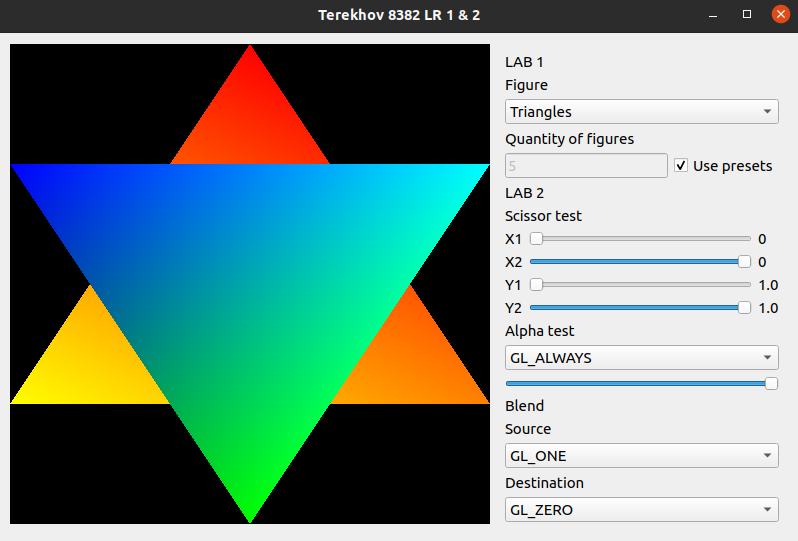
\includegraphics[width=10cm]{1}
    \caption{Интерфейс}
    \label{fig:1}
\end{figure}

Справа предусмотрена область, в которой можно настроить отображение.
Первые 4 слайдера позволяют указать границы для отсечения по горизонтали $(x_1, x_2)$ и по вертикали $(y_1, y_2)$.
В следующем списке можно выбрать параметр для теста прозрачности, и слайдером выбрать значение альфа.
Затем следуют два списка, в которых можно выбрать параметры для sfactor и dfactor соответственно.
Примеры работы программы представлены на рисунках 2-6.

\textit{Тест отсечения}
\begin{figure}[H]
    \centering
    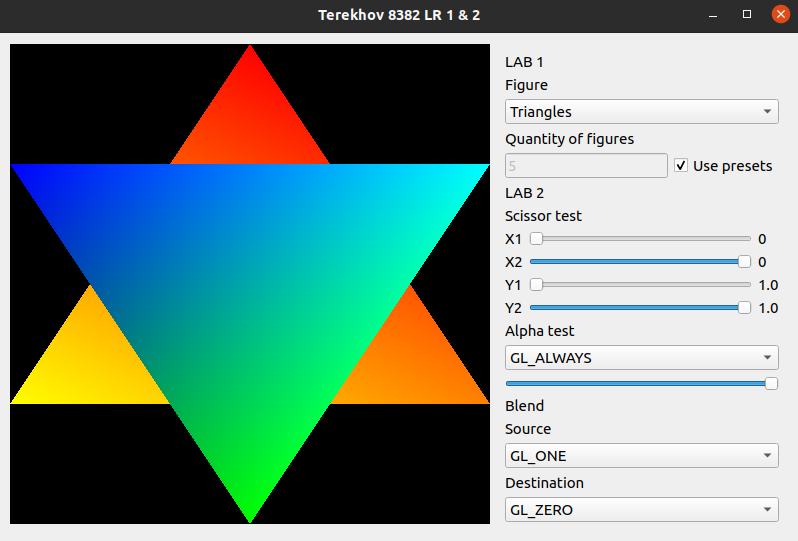
\includegraphics[width=10cm]{1}
    \caption{Исходное изображение}
    \label{fig:2}
\end{figure}
\begin{figure}[H]
    \centering
    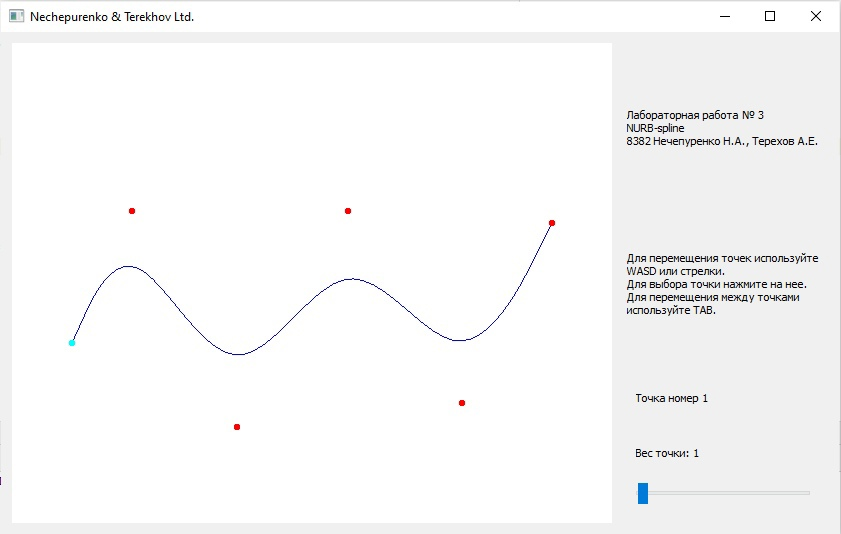
\includegraphics[width=10cm]{2}
    \caption{Результат отсечения}
    \label{fig:3}
\end{figure}
\begin{figure}[H]
    \centering
    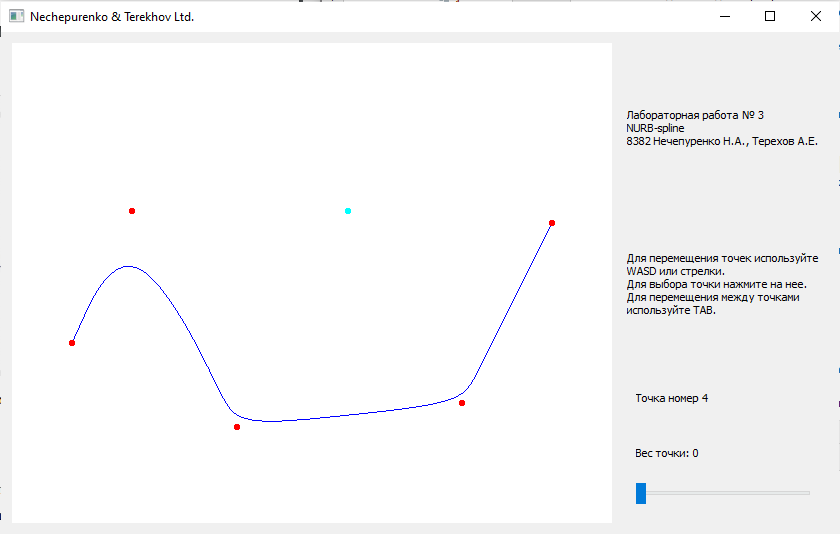
\includegraphics[width=10cm]{3}
    \caption{Результат теста прозрачности}
    \label{fig:4}
\end{figure}
\begin{figure}[H]
    \centering
    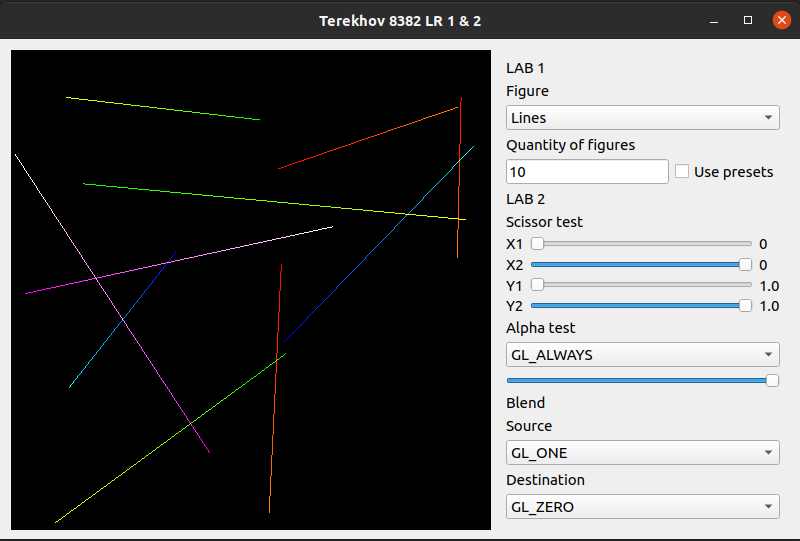
\includegraphics[width=10cm]{4}
    \caption{Результат смешения цветов с параметрами GL\_ONE, GL\_ONE}
    \label{fig:5}
\end{figure}
\begin{figure}[H]
    \centering
    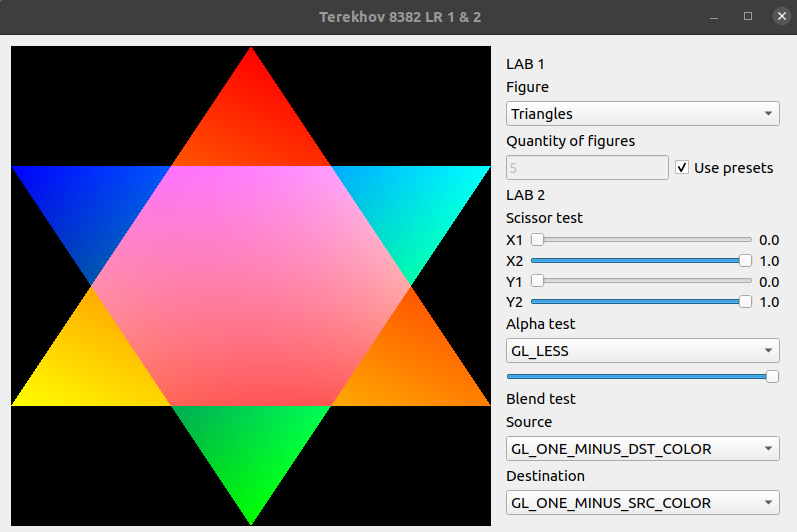
\includegraphics[width=10cm]{5}
    \caption{Результат смешения цветов с параметрами GL\_ONE\_MINUS\_DST\_COLOR, GL\_ONE\_MINUS\_SRC\_COLOR}
    \label{fig:6}
\end{figure}

\section*{Вывод}
В ходе лабораторной работы была написана программа, реализующая представление определенного набора примитивов из имеющихся в библиотеке OpenGl.
Также в программе, при помощи функций glScissor, glAlphaFunc и glBlendFunc, можно применять тесты отсечения прозрачности и смешения цветов, варьируя параметры.
Программа работает корректно.
При выполнении работы были приобретены навыки работы с графической библиотекой OpenGL.